%!TEX root = main.tex

Suponga que una fuente genera dígitos binarios con distribución uniforme, los mensajes son enviados a través de un canal cambia los símbolos que genera una fuente binaria con las probalidades que se muestran en la gráfica.\\
\begin{center}
     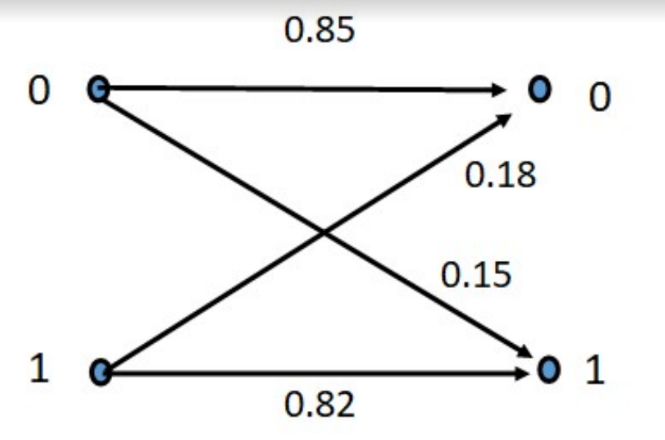
\includegraphics[scale=0.4]{punto1.png}
    \end{center}
Responda cada una de las siguientes preguntas justificando su razonamiento:\\
\textbf{a).} ¿Cuál es el número más probable de errores que se puede encontrar en un mensaje de 5000 bits que pase por el canal?\\
\begin{sol}
   Teniendo en cuenta que al evaluar si un bit fue bien codificado através del canal, el resultado que ponemos obtener es sí o no, podemos resolver este ejercicio utilizando la distribución binomial.\\
   Sabemos que, los bits pueden tomar valores de $0$ o $1$, sin embargo, el enunciado nos dice que la manera en la que se distribuyen através de los 5000 bits es uniforme, es decir, que podemos tomar la probabilidad de que el bit sea 0 o 1 como $\dfrac{1}{2}.$ \\
   Ahora bien, para calcular cada uno de los errores tomamos en cuenta la información del gráfico, así obtenemos que
   \begin{align*}
       P(0|1)=0.18\\
       P(1|0)=0.15
   \end{align*}
Por lo cual, el error total al codificar es 
\begin{align*}
    P(error)=\dfrac{1}{2}\cdot 0.18+\dfrac{1}{2}\cdot 0.5=0.165
\end{align*}
Luego, al calcular la esperanza tenemos que la cantidad de errores es
\begin{align*}
\mu=5000\cdot 0.165=825
\end{align*}
Con lo cual podemos decir que el número más probable de errores es 825.
\end{sol}
\textbf{b).} Si se codifica cada bit que genera la fuente triplicandolo, en qué porcentaje se reduce el número de errores? Suponga que para la decodificación se usa mayoría de bits por tripla.\\
\begin{sol}
   Ahora, tenemos que calcular el error para una fuente que triplica los bits, sabemos que mediante esta codificación para que se de un error quiere decir que 2 o 3 bits al pasar por el canal se codificaron de manera incorrecta. Así que calculemos esa probabilidad
   \begin{align*}
    P(errortripla)=P(2errores)+P(3errores)
    \end{align*}
    Al igual que en el numeral anterior, vamos a utilizar la  distribución binomial para calcular la probabilidad de que cambien 2 o 3 bits
    \begin{align*}
    P(\text{2 errores})&= \binom{3}{2} p^2 (1-p)=3\cdot (0.165)^{2}(0.835)=0.0681986\\
    P(\text{3 errores})&= \binom{3}{3} p^2 (1-p)= (0.165)^{3}=0.004492
    .\end{align*}
Luego el error por tripla tenemos que es 
\begin{align*}
    P(errortripla)&=P(2errores)+P(3errores)\\
    &=0.0681986+0.004492\\
    &=0.0726906
.\end{align*}   
Por lo cual tenemos que la reducción porcentual del error es
\begin{align*}
   Reducción porcentual=\dfrac{0.165-0.0726906}{0.165}\cdot 100=55.9451\%
.\end{align*}
\end{sol}
\textbf{c).} Si se codifica cada bit que genera la fuente con una n-tupla y se usa mayoría de bit por n tupla en la decodificación, cuál sería la longitud
mínima n - tupla para obtener por lo menos un 95 $\%$ de certeza en la decondificación?
\begin{sol}
  Para realizar este ejercicio tenemos que tener en cuenta que $n$ para que el criterio se decidible debe ser impar y por el numeral anterior tenemos cuando $n=3$ el error es de $7.269\%$, como estamos buscando que el error sea de $5\%$ o menor vamos a probar los siguientes casos
  \begin{itemize}
    \item \textbf{ Caso $n=5$}
    Para este caso vamos a aplicar la distribución de binomial ahora tomando los casos donde se presenten por lo menos 3 errores, asi calculamos lo siguiente
    \begin{align*}
    P(\text{3 errores}) &= \binom{5}{3} p^3 (1-p)^{5-3}=10 (0.165)^3 (0.835)^{5-3}=0.0313202, \\
    P(\text{4 errores}) &= \binom{5}{4} p^4 (1-p)^{5-4}=5(0.165)^4 (0.835)^{5-4}=0.00309451, \\
    P(\text{5 errores}) &= \binom{5}{5} p^5 (1-p)^{5-5}=(0.165)^5 (0.835)=0.000122298
\end{align*}
Entonces,tenemos que el error del código que generan las $5-$tuplas es 
\begin{align*}   
   P(5tuplaserror)&=P(\text{3 errores})+ P(\text{4 errores})+ P(\text{5 errores})\\
&= 0.0313202+0.00309451+0.000122298\\
&=0.034537
.\end{align*}


  \end{itemize}

Luego el error es de $3.4537\%$ y por lo tanto la longitud mínima para que la certeza sea de $95\%$ es de 5.



\end{sol}
